\chapter{Resultados y conclusiones}
%%
\section{Resultados}
DBCASE permite realizar el proceso de diseño y creación de una base de datos de forma sencilla mediante una interfaz de escritorio, centrándose en ayudar al estudiante en su proceso de aprendizaje.\\

%%%%%%%%%
\subsection*{Espacio de trabajo}
El usuario puede modificar muchos aspectos del espacio de trabajo para hacer más cómoda su experiencia con la aplicación.\\

Puede escoger el idioma, el tema y la perspectiva que desee. También puede redimensionar los paneles para adaptarlos a sus necesidades.
\begin{figure}[H]
    \centering
    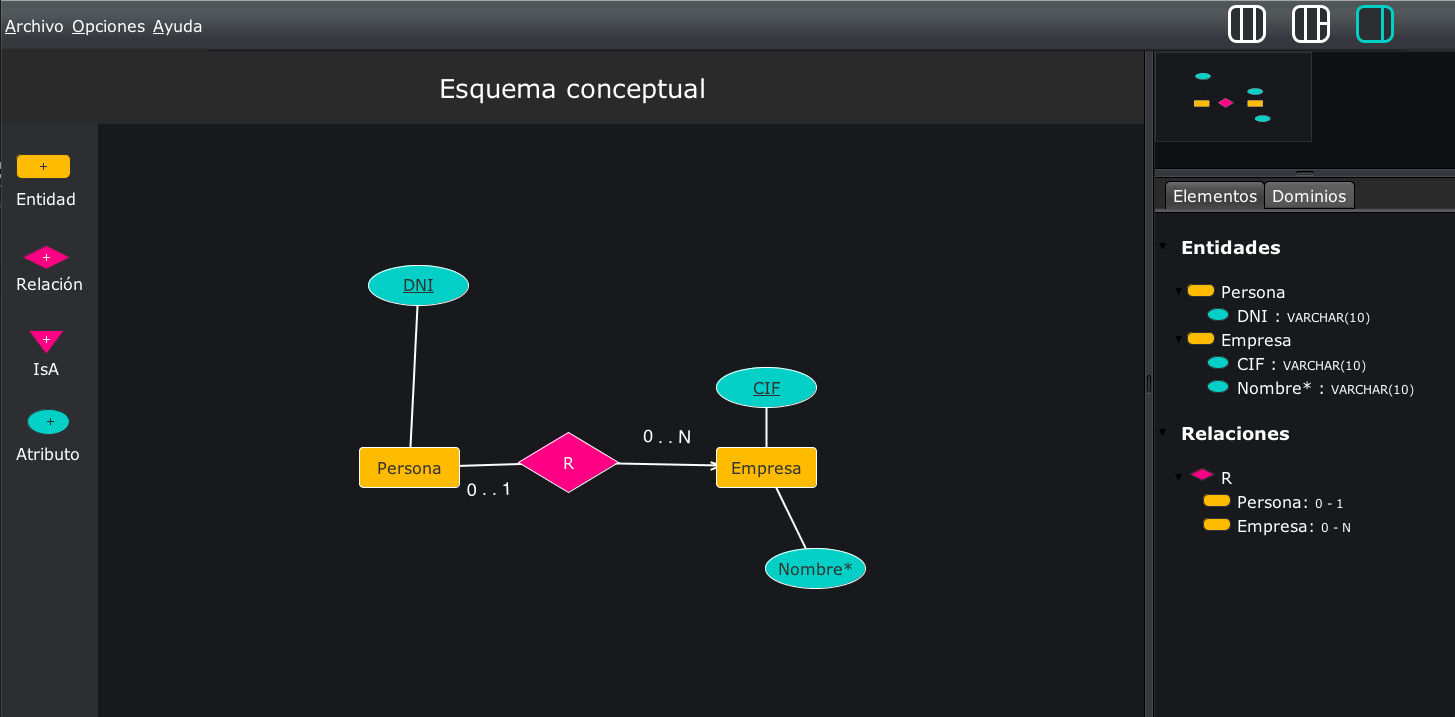
\includegraphics[width=1\textwidth]{img/black.png}
    \caption{Ejemplo de espacio de trabajo personalizado}
\end{figure}

%%%%%%%%%
\subsection*{Creación de un diagrama}
El primer paso es la creación y el diseño de un diagrama entidad relación. Para ello se debe seleccionar una de las dos perspectivas que muestran el panel de diseño.\\

Para añadir elementos al diagrama el usuario dispone de dos opciones.
\begin{itemize}
    \item Haciendo clic derecho sobre el panel de diseño. Se mostrará un menú desplegable que permite insertar cualquier tipo de elemento.
    \item Utilizando la barra lateral, pulsando en los iconos que representan los elementos.
\end{itemize}
A la hora de insertar elementos, se pueden escoger mediante distintos cuadros de diálogo las características de los mismos. Por ejemplo en el caso de insertar una nueva entidad se debe indicar el nombre, y se da la opción de que la entidad sea débil con respecto a otra existente en el diagrama. En tal caso se debe seleccionar esa entidad fuerte y dar nombre a la relación que las une.\\

El procedimiento para eliminar elementos del diagrama es el siguiente:
\begin{itemize}
    \item primero se debe seleccionar un elemento o un conjunto de elementos (bien abarcando todos los elementos con el ratón o bien seleccionando de uno en uno y manteniendo pulsada la tecla shift).
    \item Tras realizar la selección se puede eliminar los elementos de dos formas:
    \begin{itemize}
        \item Hacer clic derecho sobre el elemento, tras lo cual se mostrará un menú desplegable, en el que una de las opciones es la de eliminar el elemento.
        \item Pulsando la tecla de suprimir.
    \end{itemize}
    Antes de finalizar el proceso se mostrará un cuadro de confirmación.
\end{itemize}

%%%%%%%%%
\subsection*{Relaciones}
Uno de los elementos básicos en los diagramas entidad relación son las relaciones entre entidades.\\

Para conectar una relación con una entidad el usuario debe hacer clic derecho sobre la relación y pulsar en la opción \enquote{añadir una entidad} del menú desplegable. Tras ello se abrirá un cuadro de diálogo en el que se debe seleccionar la entidad y elegir con qué cardinalidad se desea establecer el vínculo. También se da la posibilidad de indicar un nombre para el rol del enlace.

%%%%%%%%%
\subsection*{Restricciones}
El usuario puede añadir restricciones a cualquier elemento del diagrama. Estas restricciones serán importantes a la hora de crear el script sql que genere la base de datos.\\

Para insertar restricciones a los elementos el usuario debe pulsar clic derecho sobre un elemento del diagrama y pulsar \enquote{restricciones} dentro del menú desplegable.\\

Tras ello se abrirá un cuadro de diálogo que permite al usuario crear una lista con las restricciones para ese elemento.

%%%%%%%%%
\subsection*{Dominios}
Al crear un atributo el usuario debe indicar qué dominio está vinculado con ese atributo. Aunque en un diagrama entidad relación no es necesaria esta información, sí que es importante a la hora de generar el esquema físico ya que todas las columnas de una tabla deben tener un dominio.\\

El programa ofrece por defecto once de los dominios más comúnmente usados pero también da la posibilidad al usuario de crear su propios dominios.
\begin{itemize}
    \item Pulsando clic derecho sobre un espacio vacío en el diagrama y pulsando en la opción \enquote{crear dominio}.
    \item Seleccionando la pestaña de dominios y haciendo clic en el botón de \enquote{nuevo}.
\end{itemize}
Tras ello se abre un cuadro de diálogo en el que el usuario debe indicar el nombre del dominio, el tipo base, y los valores que puede adoptar separados por comas.
%%%%%%%%%
\subsection*{Generación de códigos}
El siguiente paso tras el diseño del diagrama entidad relación es la generación de los esquemas lógico o físico.\\

Para ello el usuario debe pulsar en los botones de generar dispuestos en ambos paneles. De existir errores o advertencias, los paneles informarán de forma clara de qué se trata.\\

Una vez generados los códigos, el usuario tiene la opción de editarlos para añadir, modificar o eliminar cualquier cuestión. Una vez el usuario esté satisfecho con el código, tiene la posibilidad de exportarlo a un archivo en formato texto, o también en formato sql en el caso del esquema físico.\\

El programa también da la posibilidad de ejecutar el esquema físico directamente en el gestor de base de datos que haya seleccionado.
%%
\section{Discusión y conclusiones}%[SPA-ENG]
\textit{[ESP]}\\
La aplicación ha mejorado enormemente el aspecto gráfico y se ha adaptado en la medida de lo posible a los estándares de diseño de hoy en día. Una de las limitaciones que se ha sufrido es la de arrastrar las librerías de Jung \cite{jung} y la implementación de la interfaz mediante java swing. Hubiese sido muy interesante haber creado una nueva interfaz usando las opciones que proporciona java FX.\\

También hubiese sido interesante generar el diagrama usando otra librería distinta a Jung, ya que durante todos estos años han surgido mejores soluciones para la creación de este tipo de diagramas.\\

Al tratarse de un proyecto individual y al ser el principal objetivo hacer que la aplicación volviese a ser usable se decidió centrar los esfuerzos en ello, manteniendo por tanto las librerías de la anterior versión.\\

También se ha mejorado la funcionalidad de la aplicación corrigiendo errores, mejorando sobre todo el esquema lógico y añadiendo nuevas funcionalidades a la aplicación.\\

En lo personal, el proyecto me ha permitido aprender en profundidad cómo es el desarrollo de una aplicación de escritorio, así como aumentar mis conocimientos sobre el lenguaje java y sobre la programación orientada a objetos. Especialmente he aprendido a como construir una interfaz de usuario completa y funcional.\\

\textit{[ENG]}\\

The application has greatly improved the graphic user interface and adapted as far as possible to the design standards of today. One of the limitations that has been suffered is having to use the Jung \cite{jung} and java swing libraries. It would have been interesting to have created a new interface using the options provided by Java FX.\\

It would also have been interesting to generate the diagram using another library other than Jung, since during all these years better solutions for the creation of such diagrams have emerged.\\

Being an individual project and being the main objective to make the application usable again, it was decided to focus efforts on it, thus maintaining the libraries of the previous version.\\

The functionality of the application has also been improved by correcting errors, especially improving the logical schema and adding new functionalities to the application.\\

Personally, the project has allowed me to learn in depth how is the development of a desktop application, as well as increase my knowledge about java language and object-oriented programming. I especially learned how to build a complete and functional user interface.\\

